\chapter{Formatting Figures and Tables}
\label{ch:conclusion}

This Chapter provides examples of formatting Figures and Tables. 

\section{Formatting figures}
An example of how to format several drawings in one figure is provided on Figure~\ref{fig:QQ_different_weights}.
\begin{figure}[!htb]
\centering
\subfloat[Caption of Figure - a]{
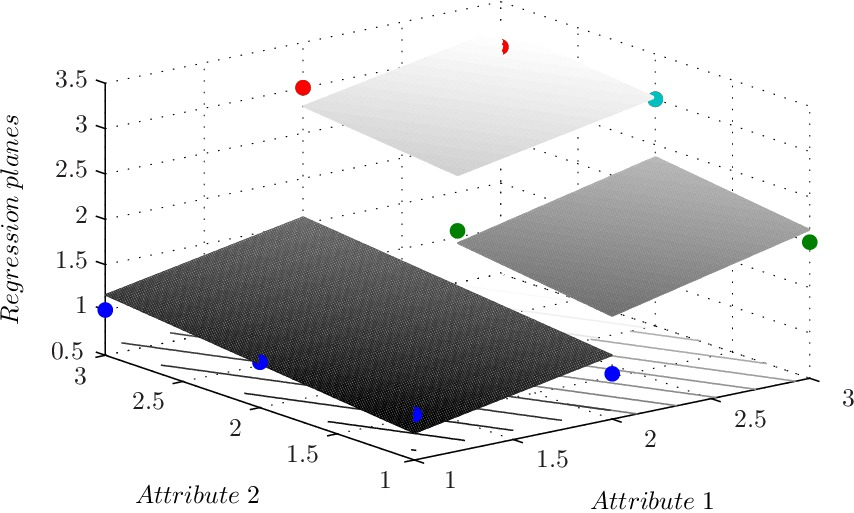
\includegraphics{./figures/chapter3/imga.jpg}
\label{fig:QQ_ginibrei}
}
\\
\subfloat[Caption of Figure - b]{
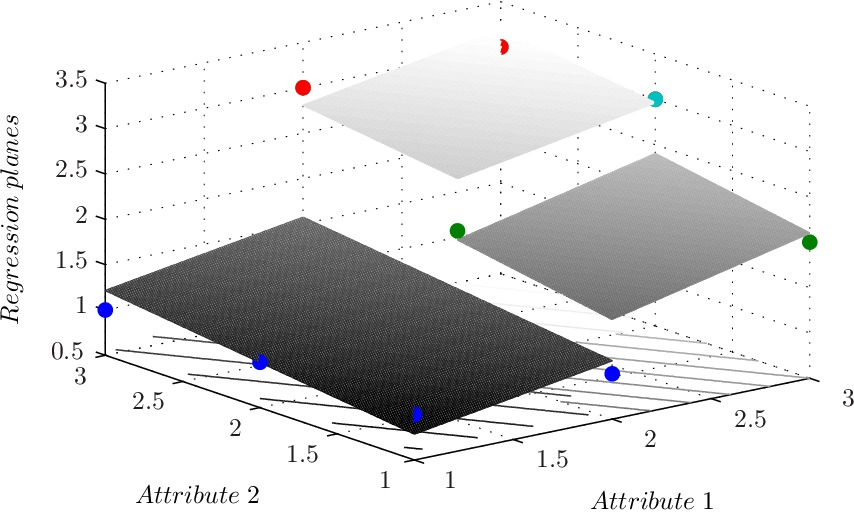
\includegraphics{./figures/chapter3/imgb.jpg}
\label{fig:QQ_ginicov}
}
\quad
\subfloat[Caption of Figure - c]{
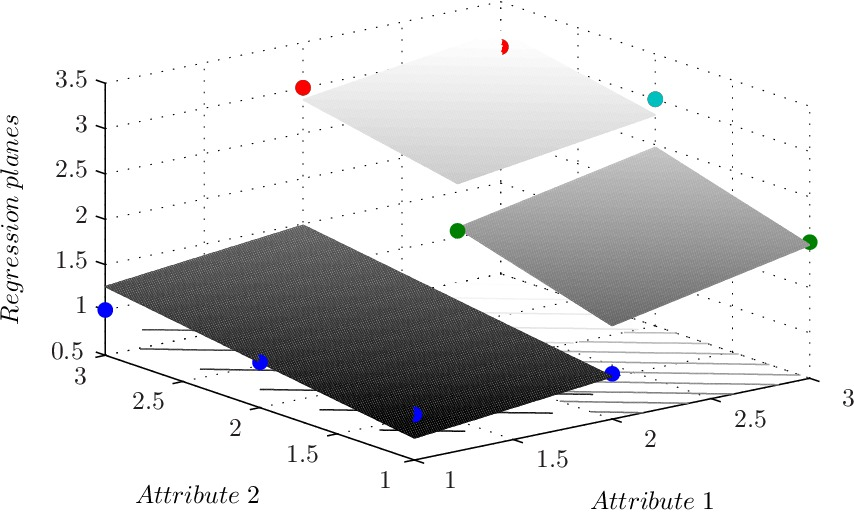
\includegraphics{./figures/chapter3/imgc.jpg}
\label{fig:QQ_ginipop}
}
\caption{Caption of the Figure}
\label{fig:QQ_different_weights}
\end{figure}


\subsection{Subsection}
\label{sec:subsection}
This is an example of subsection.

\paragraph{This is a pragraph}
This is an example of a paragraph within the subsection~\ref{sec:subsection}.

\subsubsection{Subsubsection}
This is an example of subsubsection. The maximal depth of numbered subsections is 2.

\section{Formatting Tables}
An example of how to format a table is given in Table~\ref{tbl:QQqual}. Shadings are not a requirement.

\begin{table}[!ht]
\centering
\caption{Qualitatively described problem}
\begin{tabular}{cccc}
\toprule 
\textbf{No.} & ${{\mathbf {QA}}}_{{\mathbf 1}}$\textbf{} & ${{\mathbf {QA}}}_{{\mathbf 2}}$\textbf{} & 		\textbf{QC} \\
\midrule
1 & good & good  & good \\ 
2 & better & good & good \\ 
3 & good & better & good \\ 
4 & good & the best & good \\ 
\rowcolor[gray]{0.9} 5 & the best & good & better\\ 
\rowcolor[gray]{0.9} 6 & better & better & better \\ 
7 & the best & better & the best \\ 
8 & better & the best & the best \\ 
9 & the best & the best & the best \\ 
\bottomrule 
\end{tabular}
\label{tbl:QQqual}
\hspace{0.5cm}
\end{table}


%
% In order to color the first row cell/-s, \rowcolor[gray]{0.9} is used.
% The word 'gray' here denotes the grayscale color scheme, not the color grey and `0.9' denotes how dark the grey is.
%
% The xcolor package provides the necessary commands to produce tables with alternate row colors, when loaded with the table option.
% The command \rowcolors{<starting row>}{<odd color>}{<even color>} has to be specified right before the tabular environment starts.
%
% For footnotes to work inside of tables, apply minipage environment before entering tabular environment.

